\chapter{Method}
\begin{figure}[h]
	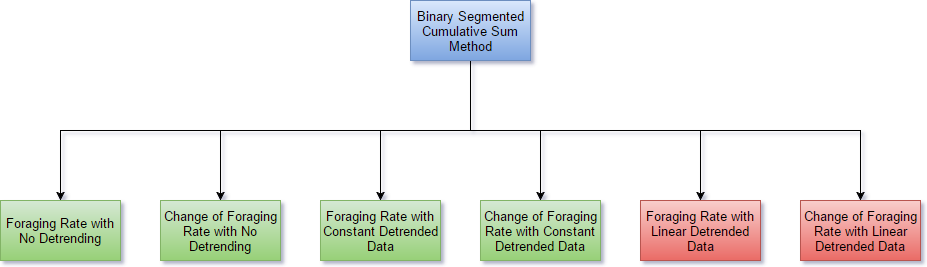
\includegraphics[width=\textwidth]{ChangePoint.png}
	\caption{Steps of Change Point Analysis}
\end{figure}
\section{\label{section:Setting Simulation Environment}Setting Simulation Environment}
We tried to setup the simulation environment as like as the field experiment environment. So we distributed the resources in Donut Shapes. We had three different setups for three different species of ants. For \textit{Rugosus} the distribution of the resources was in power law and the power rank was $5$. Total $1024$ seeds are distributed in 4 different densities. $256$ seeds are piled up in one single pile. There were $4$ piles of $64$ seeds in each. $16$ piles had $16$ seeds each and rest of the $256$ seeds were distributed uniformly among the nest in the donut shape ring. Although in the field experiment, the area of the donut shape was proportional to the colony size. In here we tried to keep the area of the donut shape ring constant. The inner radius of the ring was $5$ meter and the outside radius was $10$ meter. The total duration of each experiment was $90$ minutes (We collected data from field experiments for $90$ minutes only). The total arena size was $20\times20$ meter. We kept the arena into this size and bounded the agents to search in this arena.  The setup is varied for \textit{Maricopa} and \textit{Desertorum}. The following table represents the environmental setup of simulations for \textit{P. Rugosus}, \textit{P. Maricopa} \& \textit{P. Desertorum}.
\begin{table}
	\begin{tabular}{ |p{0.3\textwidth}|p{0.3\textwidth}|p{0.3\textwidth}| } 
		\hline
		\textbf{Species} & \textbf{Number of Seeds} & \textbf{Radius of Seed Distribution} \\
		\hline 
		\textit{P. Rugosus} & 1024 & 5-10 meter\\ 
		\hline
		\textit{P. Maricopa} & 128 & 1-3 meter\\ 
		\hline
		 \textit{P. Desertorum} & 128 & 1-3 meter\\
		\hline
	\end{tabular}
	\caption{Environmental Setup of simulation for three species}
\end{table}
\begin{figure}[h]
	\frame{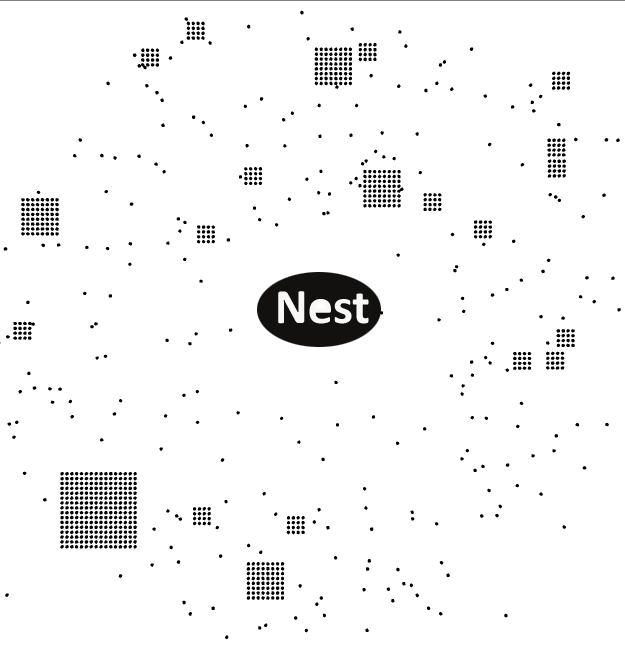
\includegraphics[width=\textwidth]{ArGOS.jpg}}
	\caption{Example setup of a simulation environment for \textit{P. Rugosus}. The setup showing three different types of piles. One large pile of $256$ seeds, Four piles of $64$ seeds and sixteen piles of $16$ seeds. $256$ random seeds are distributed uniformly inside the ring. }
\end{figure}
\section{\label{section:overview}Overview}
   The classic approach to proving a theorem is some really difficult 
   mathematics.  For the theory of relativity, I asked grandpa Al exactly 
   how he proved it.  He gave me a few hints, including some stuff about
   rest mass and big electro-motive force.  I think he is really smart.
\section{Conclusions}
   I conclude that this is a really short thesis.